\chapter{Strømforsyning}
Ud fra kravspecifikation skal delmodulerne (SM og VBTE) kunne drives fra en 24V AC/DC forsynings kilde. Selve modulerne er designet til 12V DC og 5V DC forsyningsspændringer , der designes derfor en strømforsyning der regulere spændingen så den kan levere 12V 1A og 5V 0,5A.  

\section{Overordnet design}
I dette afsnit beskrives og vises det overordnede hardware blokdiagram over strømforsyningen samt beskrivelse signaler.
\begin{figure}[H]
\centering
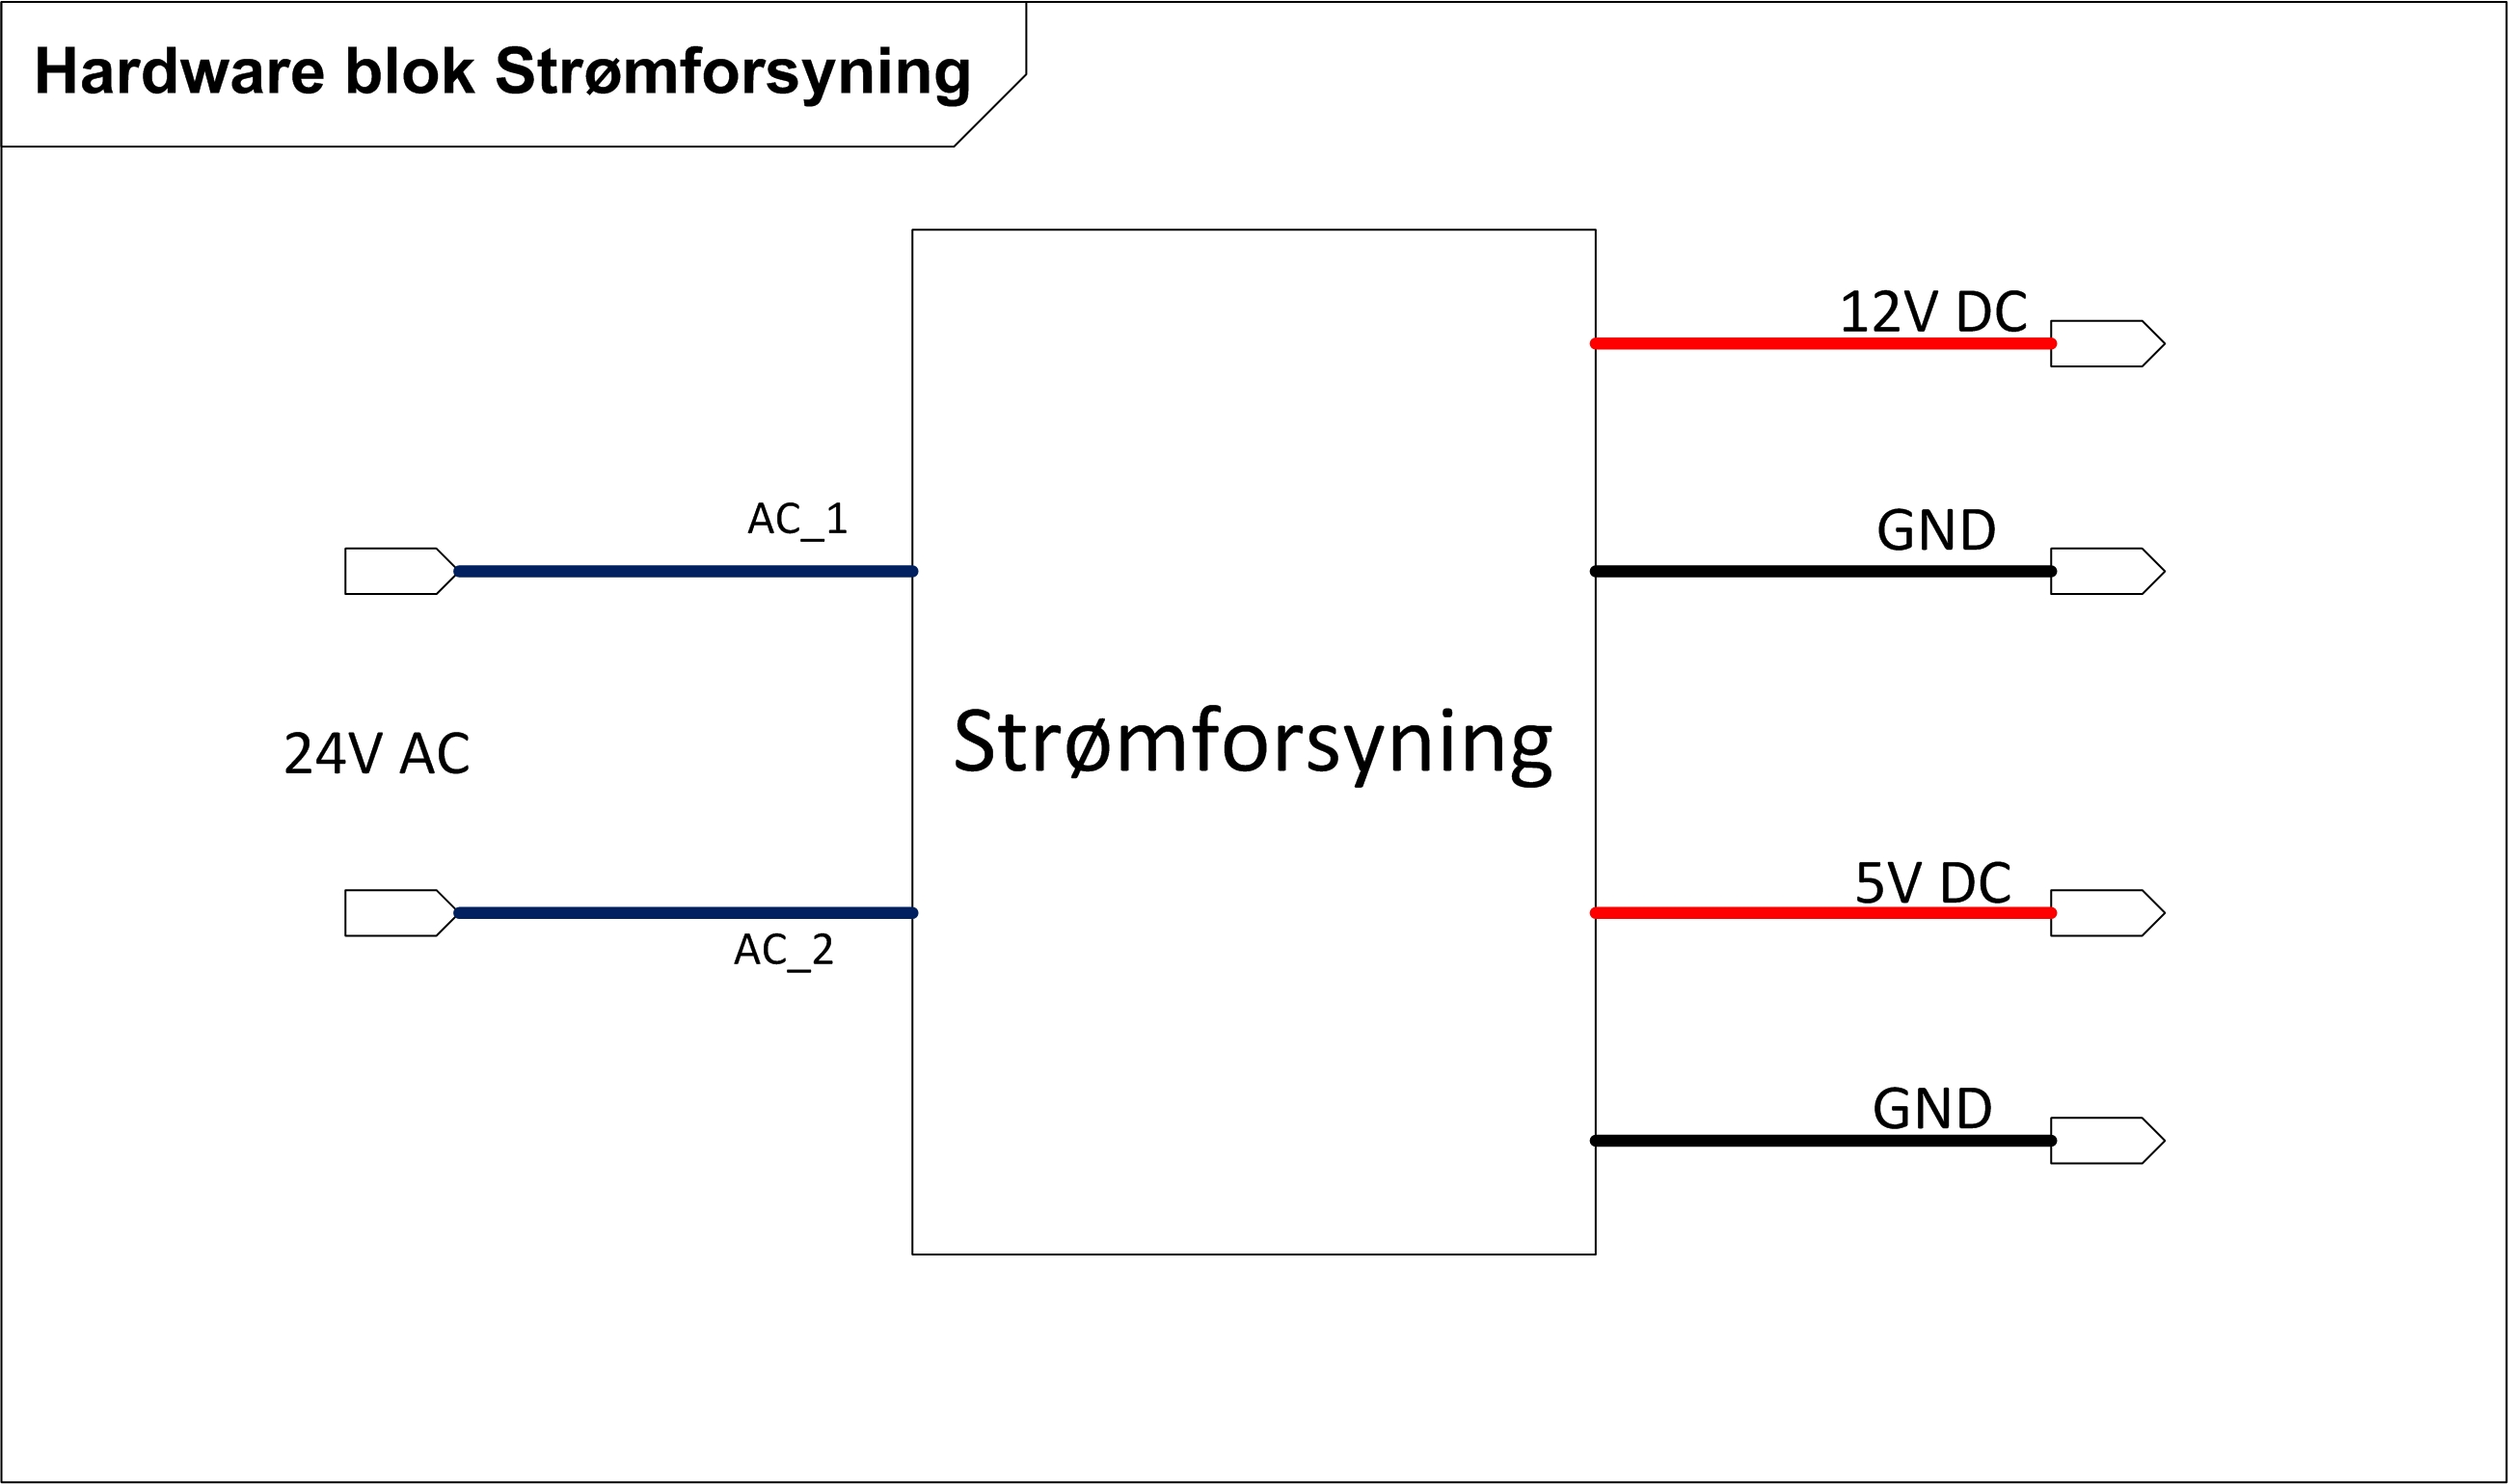
\includegraphics[scale=0.6]{billeder/PowerSupply}
\caption{Strømforsyning}
\label{fig:PowerSubbly}
\end{figure}
\begin{figure}[H]
\centering
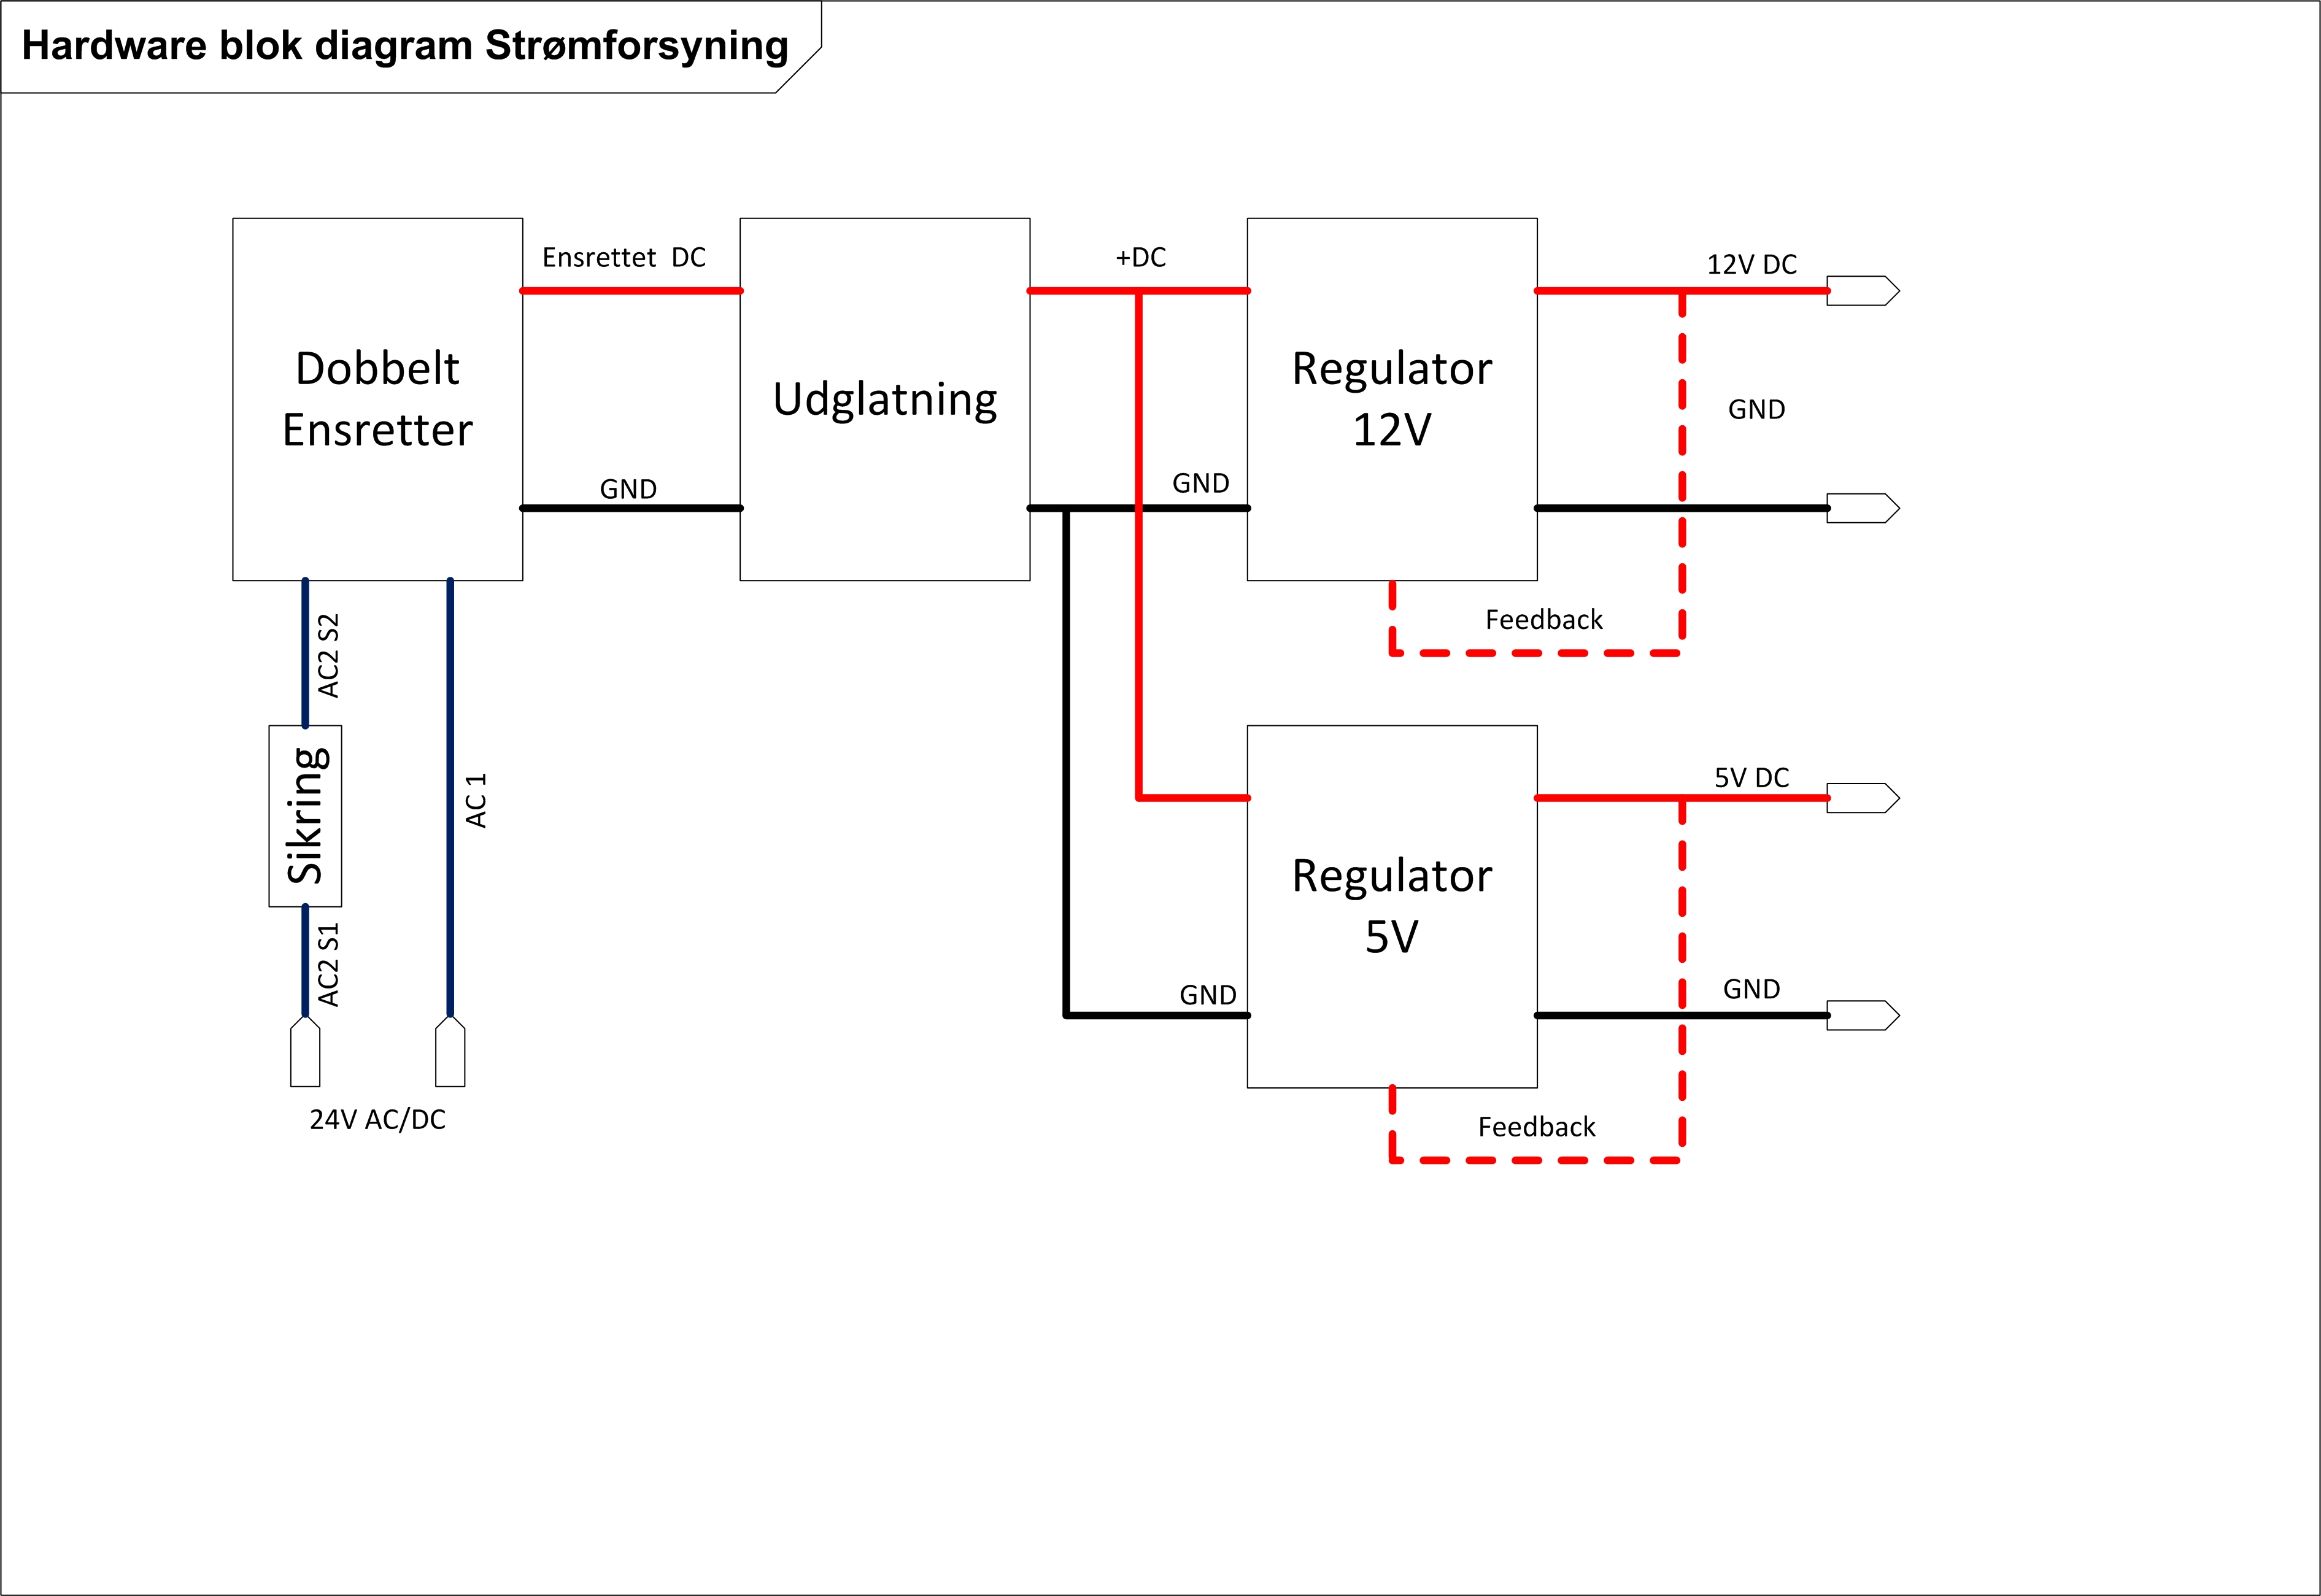
\includegraphics[scale=0.8]{billeder/PowerSupplyBlok}
\caption{Overordnet blokdiagram for strømforsyning}
\label{fig:PowerSubbly Blok}
\end{figure}
\newpage
\subsection{Blokke}
Nedenfor beskrives de enkelte blokke illustreret på \textit{Figur~\ref{fig:PowerSubbly Blok}}
\subsubsection{Sikring}
Sikringen beskytter forsyningskilde, hvis der bliver for stor belastning på strømforsyningen
\subsubsection{Dobbelt ensretter}
Ensretter AC eller DC spændingen fra forsyningskilden.
\subsubsection{Udglatning}
Udglatter det ensrettet signal til en stabil positiv DC. 
\subsubsection{Regulator 12V}
Regulere den ensrettet DC ned til 12V DC.
\subsubsection{Regulator 5V}
Regulere den ensrettet DC ned til 5V DC.
\newpage
\section{Nedbrydning af blokke}
For at gøre designet af de forskellige blokke mere overskuelig nedbrydes de enkle blokke fra det overordnede blokdiagram.
\subsection{Sikring}
\begin{figure}[H]
\centering
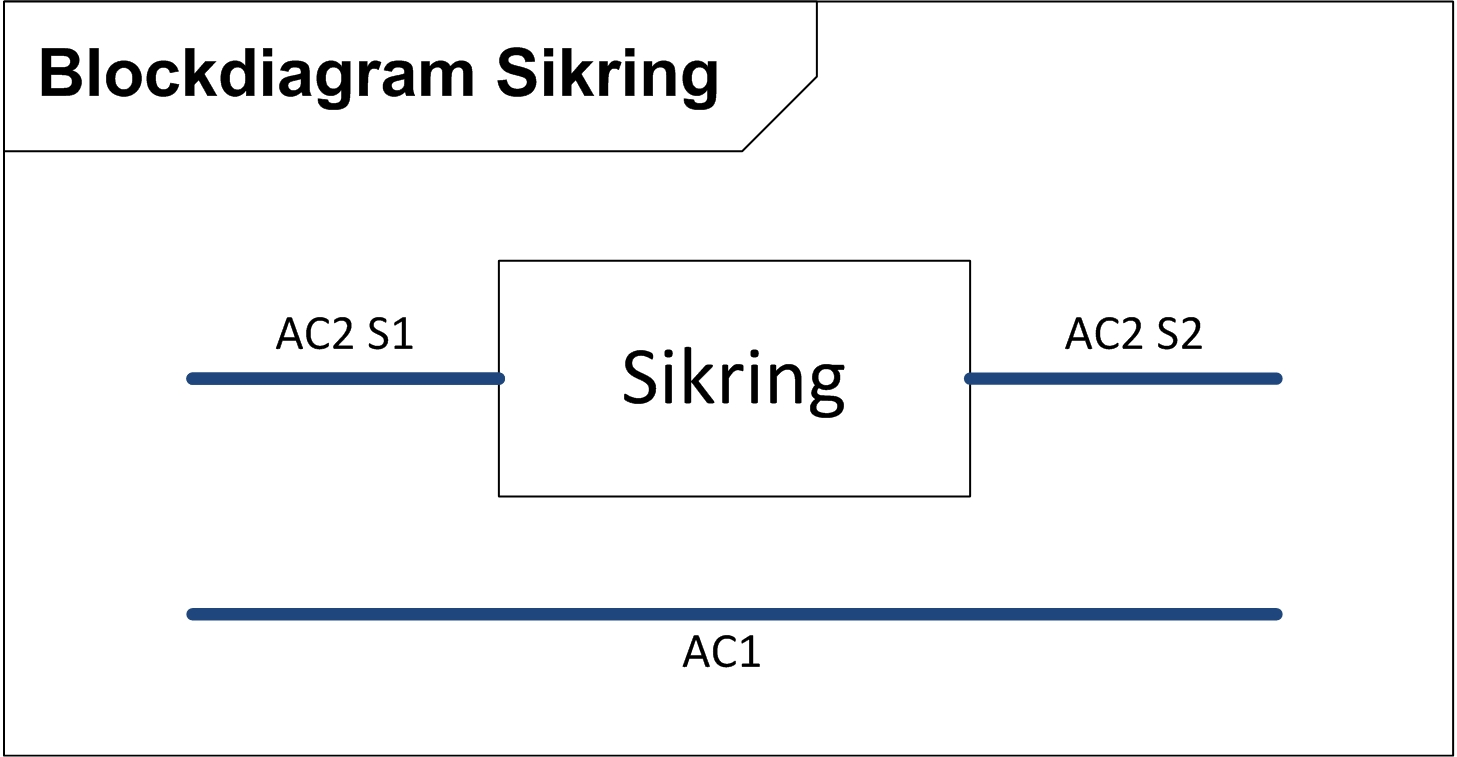
\includegraphics[scale=1]{billeder/SikringsBlok}
\caption{Blokdiagram for Sikrings blok}
\label{fig:SikringsBlok}
\end{figure}
\subsubsection{Signalbeskrivelser}
I tabellen beskrives de interne signaler
\begin{table}[H]
\begin{tabular}{|p{3cm}|p{3cm}|p{3cm}|p{4.5cm}|} \hline
\cellcolor[gray]{0.85}Signal navn& \cellcolor[gray]{0.85}Type &\cellcolor[gray]{0.85}Spænding&\cellcolor[gray]{0.85}Beskrivelse\\ \hline
AC/DC\_1 S1 & Analog  & 24V AC / 24V DC & Indgangsspænding fra spændingskilde inden sikring.\\  \hline
AC/DC\_1   & Analog & 24V AC / 24V DC & Indgangsspænding fra spændingskilde efter sikring. \\  \hline
AC/DC\_2 & Analog & 0V AC / 0V DC & 0V AC eller 0V DC fra spændingskilden.\\  \hline

\end{tabular}
\caption{Tabel over signaler i Sikring}
\label{table:SikringSignaler}
\end{table}
\newpage
\subsection{Dobbelt ensretter}
\begin{figure}[H]
\centering
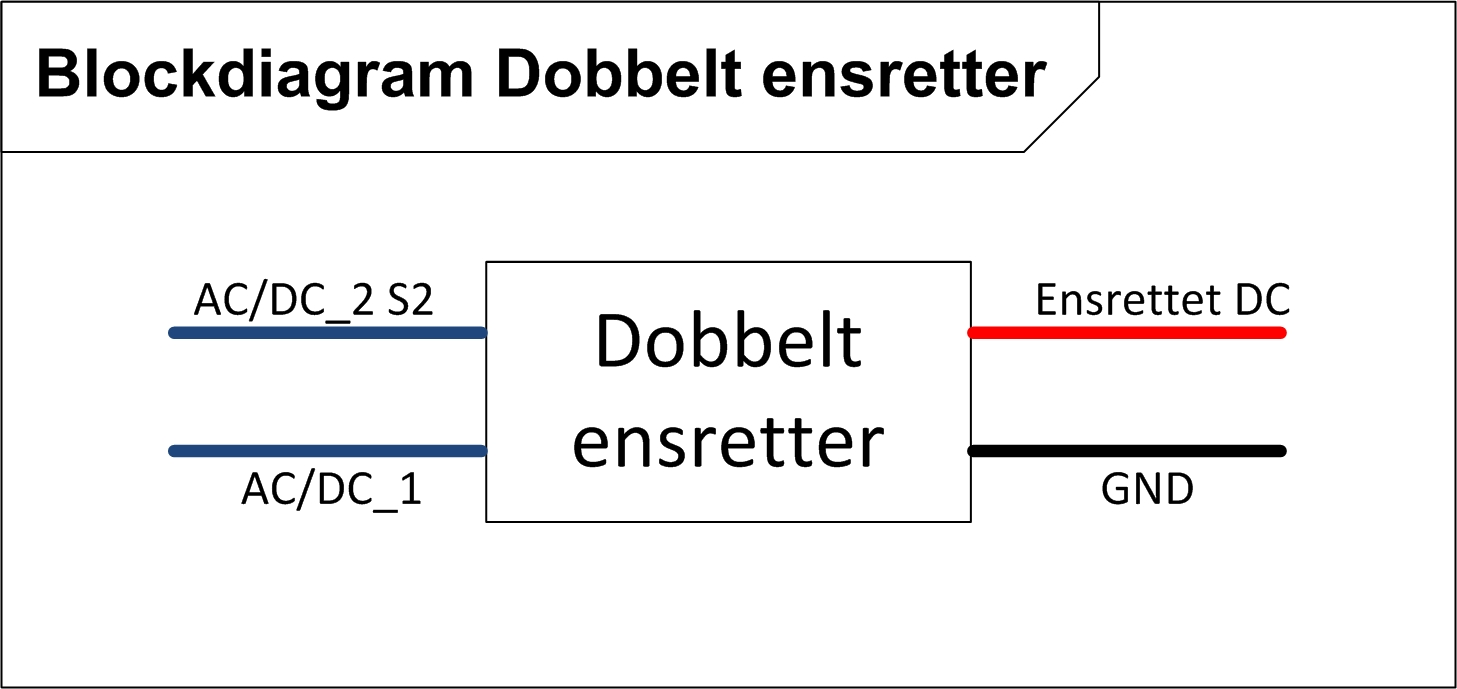
\includegraphics[scale=1]{billeder/DobbeltensretterBlok}
\caption{Blokdiagram for Dobbelt ensretter}
\label{fig:DobbeltensretterBlok}
\end{figure}
\subsubsection{Signalbeskrivelser}
I tabellen beskrives de interne signaler
\begin{table}[H]
\begin{tabular}{|p{3cm}|p{3cm}|p{3cm}|p{4.5cm}|} \hline
\cellcolor[gray]{0.85}Signal navn& \cellcolor[gray]{0.85}Type &\cellcolor[gray]{0.85}Spænding&\cellcolor[gray]{0.85}Beskrivelse\\ \hline
AC/DC\_1 S2 & Analog  & 24V AC / 24V DC & Indgangsspænding fra spændingskilde efter sikring.\\  \hline
AC/DC\_2  & Analog & 0V AC / 0V DC & 0V AC eller 0V DC fra spændingskilden. \\  \hline
Ensrettet DC & Analog & ca. 23 - 33 Vpk. & Det ensrettet signal består af positive halvbuer. Hvis DC vil der være en jævn og stabil DC.\\ \hline
GND & Analog & 0V & ground signal.\\ \hline
\end{tabular}
\caption{Tabel over signaler i Sikring}
\label{table:Ensretter}
\end{table}
\newpage
\subsection{Udglatning}
Udglatningen genere et jærn og stabilt DC-niveau
\begin{figure}[H]
\centering
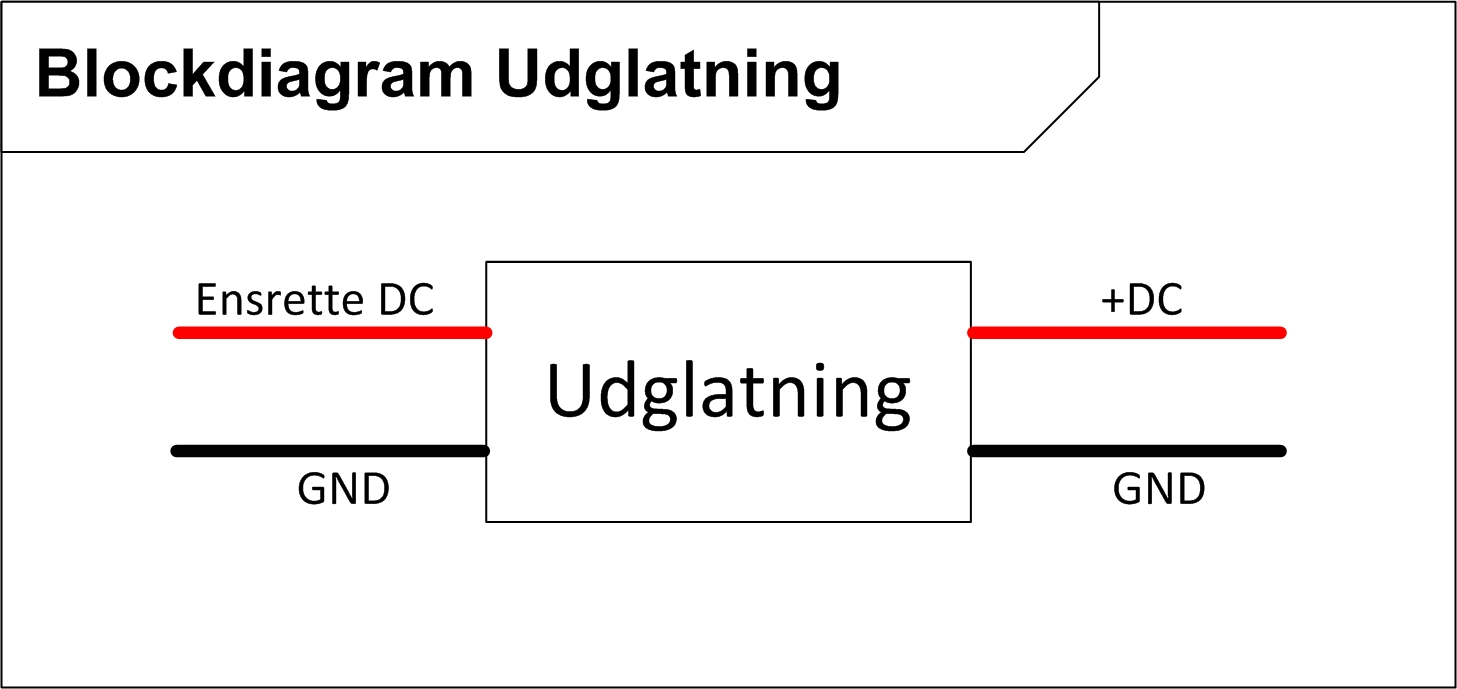
\includegraphics[scale=1]{billeder/UdglatningsBlok}
\caption{Blokdiagram for udglatning}
\label{fig:UdglatningBlok}
\end{figure}
\subsubsection{Signalbeskrivelser}
I tabellen beskrives de interne signaler.
\begin{table}[H]
\begin{tabular}{|p{3cm}|p{3cm}|p{3cm}|p{4.5cm}|} \hline
\cellcolor[gray]{0.85}Signal navn& \cellcolor[gray]{0.85}Type &\cellcolor[gray]{0.85}Spænding&\cellcolor[gray]{0.85}Beskrivelse\\ \hline
Ensrettet DC & Analog  & ca. 23 - 34 Vpk & Det ensrettet signal består af positive halvbuer. Hvis DC vil der være en jævn og stabil DC.\\  \hline
GND  & Analog & 0V DC & ground signal. \\  \hline
+DC & Analog & ca. (24V * 1.41)V DC & jævnt og stabilt DC-niveau\\ \hline
GND & Analog & 0V DC & ground signal.\\ \hline
\end{tabular}
\caption{Tabel over signaler i Udglatning}
\label{table:udglatning}
\end{table}
\newpage
\subsection{Regulator 12V}
Regulere spædning ned til 12V DC, 1A
\begin{figure}[H]
\centering
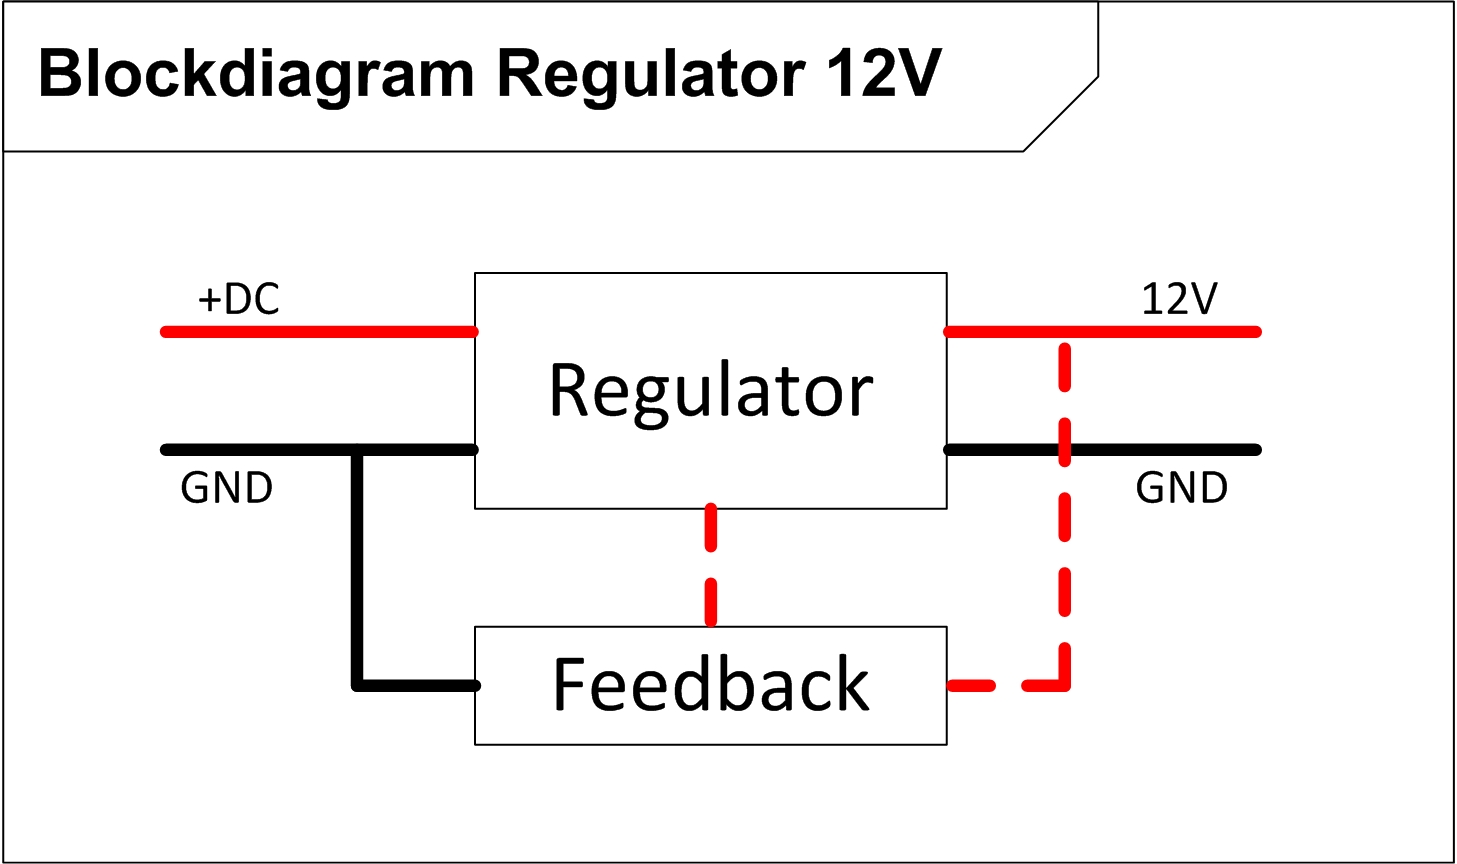
\includegraphics[scale=1]{billeder/Regulering_12VBlok}
\caption{Blokdiagram for regulator 12V}
\label{fig:regulator_12V}
\end{figure}
\subsubsection{Signalbeskrivelser}
I tabellen beskrives de interne signaler.
\begin{table}[H]
\begin{tabular}{|p{3cm}|p{3cm}|p{3cm}|p{4.5cm}|} \hline
\cellcolor[gray]{0.85}Signal navn& \cellcolor[gray]{0.85}Type &\cellcolor[gray]{0.85}Spænding&\cellcolor[gray]{0.85}Beskrivelse\\ \hline
+DC & Analog & 23 - 34 VDC & jævnt og stabilt DC-niveau\\  \hline
GND  & Analog & 0V DC & ground signal. \\  \hline
12V & Analog & 12V +-0.2V & jævnt og stabilt DC-niveau\\ \hline
GND & Analog & 0V DC & ground signal.\\ \hline
Feedback\_udgang & Analog & 12V +-0.2V & Feedback signalet måler på 12V udgangen.\\ \hline
\end{tabular}
\caption{Tabel over signaler i Sikring}
\label{table:udglatning}
\end{table}
\subsubsection{Blokbeskrivelser}
\subsubsection{Regulator}
Regulatoren regulere spænding ned til 12V, de 12V er bestemt ud fra hvad feedbacket. 
\subsubsection{Feedback}
Feedbacket måler på udgangssignalet af regulatoren, feedbacket bestemmet hvilke spændning regulatoren skal indstille sig på.
\newpage
\subsection{Regulator 5V}
Regulere spædning ned til 5V DC, 0.5A
\begin{figure}[H]
\centering
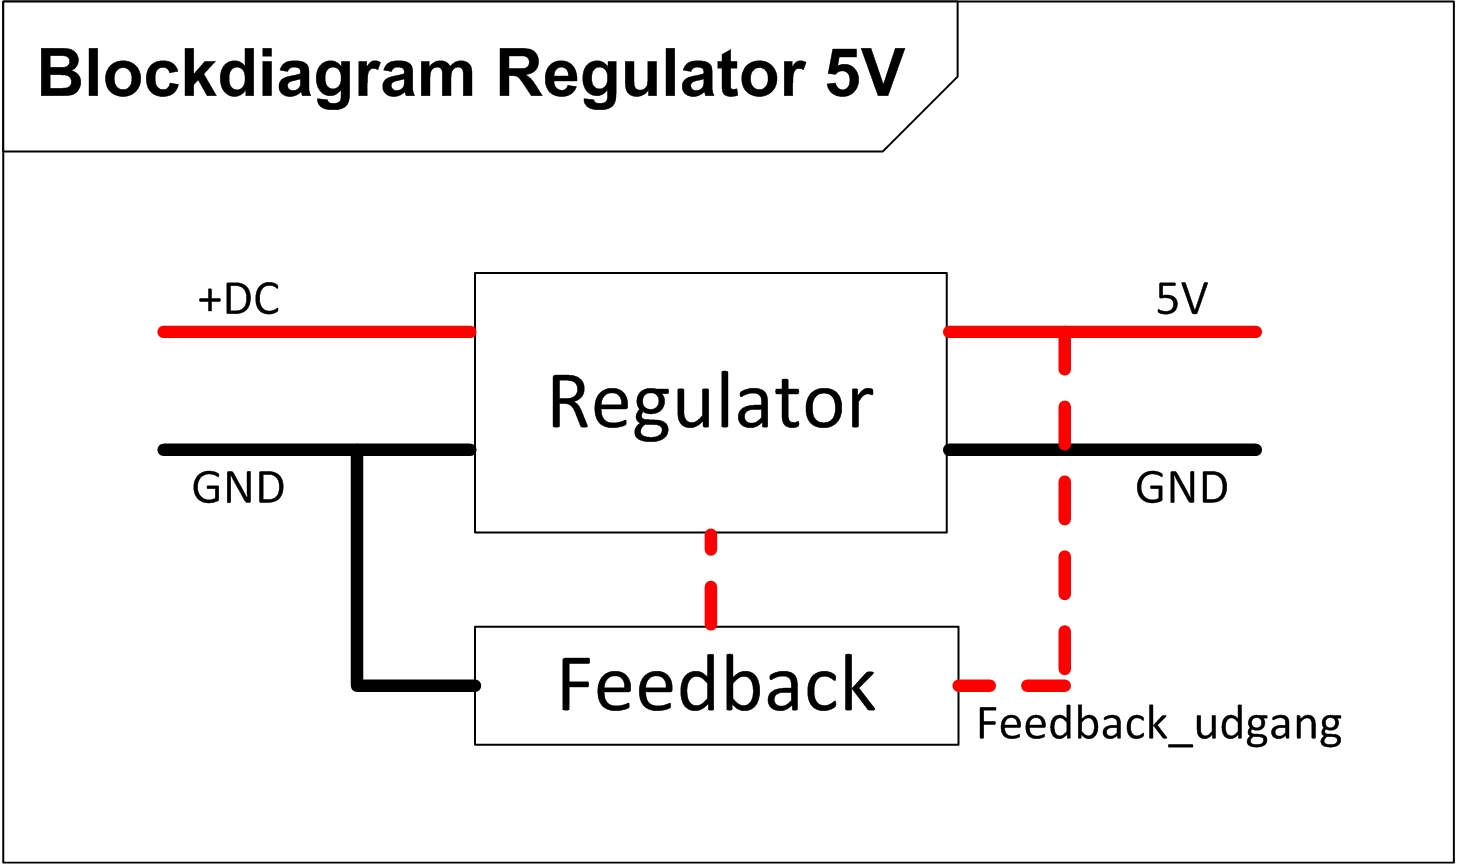
\includegraphics[scale=1]{billeder/Regulering_5VBlok}
\caption{Blokdiagram for regulator 5V}
\label{fig:regulator_5V}
\end{figure}
\subsubsection{Signalbeskrivelser}
I tabellen beskrives de interne signaler.
\begin{table}[H]
\begin{tabular}{|p{3cm}|p{3cm}|p{3cm}|p{4.5cm}|} \hline
\cellcolor[gray]{0.85}Signal navn& \cellcolor[gray]{0.85}Type &\cellcolor[gray]{0.85}Spænding&\cellcolor[gray]{0.85}Beskrivelse\\ \hline
+DC & Analog & 23 - 34 VDC & jævnt og stabilt DC-niveau\\  \hline
GND  & Analog & 0V DC & ground signal. \\  \hline
12V & Analog & 5V +-0.2V & jævnt og stabilt DC-niveau\\ \hline
GND & Analog & 0V DC & ground signal.\\ \hline
Feedback\_udgang & Analog & 5V +-0.2V & Feedback signalet måler på 12V udgangen.\\ \hline
\end{tabular}
\caption{Tabel over signaler i Sikring}
\label{table:udglatning}
\end{table}
\subsubsection{Blokbeskrivelser}
\subsubsection{Regulator}
Regulatoren regulere spænding ned til 5V, de 5V er bestemt ud fra hvad feedbacket. 
\subsubsection{Feedback}
Feedbacket måler på udgangssignalet af regulatoren, feedbacket bestemmet hvilke spændning regulatoren skal indstille sig på.
\newpage
\section{Opbygning af design}

